\documentclass[a4paper]{article}
\usepackage{amsmath}
\addtolength{\hoffset}{-2.25cm}
\addtolength{\textwidth}{4.5cm}
\addtolength{\voffset}{-3.25cm}
\addtolength{\textheight}{5cm}
\setlength{\parindent}{15pt}

\usepackage[unicode=true, colorlinks=false, hidelinks]{hyperref}
\usepackage[utf8]{inputenc}
\usepackage[english, russian]{babel}
\usepackage{mathtext}
\usepackage[T2A, TS1]{fontenc}
\usepackage{microtype} % Slightly tweak font spacing for aesthetics
\usepackage{amsthm, amssymb, amsmath, amsfonts, nccmath}
\usepackage{nicefrac}
\usepackage{epstopdf}
\usepackage[export]{adjustbox}
\usepackage{float} % Improved interface for floating objects
\usepackage{graphicx, multicol} % Enhanced support for graphics
\usepackage{pdfrender,xcolor}
\usepackage{breqn}
\usepackage{mathtools}
\usepackage{titling}
\usepackage{bm}
\usepackage{centernot}
\usepackage[cal=boondoxo,calscaled=.96]{mathalpha}
\usepackage{marvosym, wasysym} % More symbols
\usepackage{rotating} % Rotation tools
\usepackage{censor} % Facilities for controlling restricted text

\usepackage{fancyhdr}
\pagestyle{fancy}
\fancyhead{}\renewcommand{\headrulewidth}{0pt}
\fancyfoot[L]{}
\fancyhead{}
\fancyfoot{}
\fancyfoot[R]{\thepage}
\newcommand{\REALMU}{0.1272}
\newcommand{\REALSIGMA}{0.9791}
\newcommand{\MRealDistributionChiRes}{2.88}
\newcommand{\BigNK}{7}
\newcommand{\LevelAlpha}{0.05}
\newcommand{\BigChi}{12.59}
\newcommand{\MLAPLACEChiRes}{1.9}
\newcommand{\MUNIFORMChiRes}{4.44}
\newcommand{\SmallNK}{4}
\newcommand{\SmallChi}{7.81}

\begin{document}
    \begin{titlepage}
   \begin{center}
       \vspace*{3cm}
       \large{САНКТ-ПЕТЕРБУРГСКИЙ ПОЛИТЕХНИЧЕСКИЙ УНИВЕРСИТЕТ}
       \vspace{0.4 cm}

       \large\textbf{Институт прикладной математики и механики}
       \vspace{0.4 cm}

       \large{Высшая школа прикладной математики и вычислительной физики}

       \vspace{3 cm}
       \normalsize\textbf{Отчет\\ по лабораторной работе №7\\ по дисциплине\\
«Математическая статистика»}
       \vfill
       \begin{flushright}
            \normalsize{Выполнил студент:\\
            Антонов Алексей\\
            группа: 3630102/80201}
            \vskip\medskipamount
            \normalsize{Проверил:

            к.ф.-м.н., доцент\\
            Баженов Александр Николаевич
            }
       \end{flushright}

       \vspace{0.8cm}


       \normalsize{Санкт-Петербург\\2021 г.}

   \end{center}
\end{titlepage}
    \tableofcontents
    \newpage
	\listoffigures
    \newpage
	\section{Постановка задачи}
        \noindent Найти оценки коэффициентов линейной регрессии $y_{i} = a + bx_{i} + e_{i}$, используя 20 точек на отрезке [-1.8; 2] с равномерным шагом равным 0.2. Ошибку $e_{i}$ считать нормально распределённой с параметрами (0, 1). В качестве эталонной зависимости взять $y_{i} = 2 + 2x_{i} + e_{i}$. При построении оценок коэффициентов использовать два критерия: критерий наименьших квадратов и критерий наименьших модулей. Проделать то же самое для выборки, у которой в значения $y_{1}$ и $y_{20}$ вносятся возмущения 10 и -10.

    \section{Теория}
        \subsection{Простая линейная регрессия}
            \subsubsection{Модель простой линейной регрессии}
            \noindent Регрессионную модель описания данных называют простой линейной регрессией, если
            \begin{equation}
                y_{i} = \beta_{0} + \beta_{1}x_{i} + \varepsilon_{i},  i = 1..n
                \label{y_i}
            \end{equation}

            \noindent где $x_1,...,x_n - $ заданные числа (значения фактора);
            $y_1,...y_n - $ наблюдаемые значения отклика;
            $\varepsilon_1,...,\varepsilon_n - $ независимые, нормально распределенные $N(0, \sigma)$ с нулевым математическим ожиданием и одинаковой (неизвестной) дисперсией случайные величины (ненаблюдаемые);
            $\beta_0, \beta_1 - $ неизвестные параметры, подлежащие оцениванию.

            \noindent В модели (\ref{y_i}) отклик y зависит зависит от одного фактора x, и весь разброс экспериментальных точек объясняется только погрешностями наблюдений (результатов измерений) отклика y. Погрешности результатов измерений x в этой модели полагают существенно меньшими погрешностей результатов измерений y, так что ими можно пренебречь [1, с. 507].

            \subsubsection{Метод наименьших квадратов}
            \noindent При оценивании параметров регрессионной модели используют различные методы. Один из наиболее распрстранённых подходов заключается в следующем: вводится мера (критерий) рассогласования отклика и регрессионной функции, и оценки параметров регрессии определяются так, чтобы сделать это рассогласование наименьшим. Достаточно простые расчётные формулы для оценок получают при выборе критерия в виде суммы квадратов отклонений значений отклика от значений регрессионной функции (сумма квадратов остатков):
            \begin{equation}
                Q(\beta_{0}, \beta_{1}) = \sum_{i=1}^{n}{\varepsilon_{i}^{2}} =
                \sum_{i=1}^{n}{(y_{i} - \beta_{0} - \beta_{1}x_{i})^{2}}\rightarrow \min_{\beta_{0}, \beta_{1}}
                \label{Q_beta}
            \end{equation}
            Задача минимизации квадратичного критерия $Q(\beta_0, \beta_1)$ носит название задачи метода наименьших квадратов (МНК), а оценки $\hat{\beta_0}, \hat{\beta_1}$ параметров $\beta_0, \beta_1$, реализующие минимум критерия $Q(\beta_0, \beta_1)$, называют МНК-оценками [1, с. 508].

            \subsubsection{Расчётные формулы для МНК-оценок}
            \noindent МНК-оценки параметров $\hat{\beta_0}, \hat{\beta_1}$ находятся из условия обращения функции $Q(\beta_0, \beta_1)$ в минимум.
            \newline
            Для нахождения МНК-оценок $\hat{\beta_0}, \hat{\beta_1}$ выпишем необходимые условия экстремума
            \begin{equation}
               \begin{cases}
                 & \frac{\partial Q}{\partial \beta_{0}}  =
                 -2\sum_{i=1}^{n}{(y_{i} - \beta_{0} - \beta_{1}x_{i})} = 0\\
                 & \frac{\partial Q}{\partial \beta_{1}}  =
                 -2\sum_{i=1}^{n}{(y_{i} - \beta_{0} - \beta_{1}x_{i})x_{i}} = 0
               \end{cases}
               \label{sys_min}
            \end{equation}
            Далее для упрощения записи сумм будем опускать индекс суммирования. Из системы (\ref{sys_min}) получим:
            \begin{equation}
               \begin{cases}
                 & n\hat{\beta_{0}} + \hat{\beta_{1}}\sum_{}{}{x_{i}} =
                 \sum_{}{}{y_{i}}\\
                & \hat{\beta_{0}}\sum_{}{}{x_{i}} + \hat{\beta_{1}}\sum_{}{}{x_{i}^{2}} = \sum_{}{}{x_{i}y_{i}}
               \end{cases}
               \label{sys_2}
            \end{equation}
            Разделим оба уравнения на n:
            \begin{equation}
               \begin{cases}
                 & \hat{\beta_{0}} + \hat{\beta_{1}}(\frac{1}{n}\sum_{}{}{x_{i}}) =
                 \frac{1}{n}\sum_{}{}{y_{i}}\\
                & \hat{\beta_{0}}(\frac{1}{n}\sum_{}{}{x_{i}}) + \hat{\beta_{1}}(\frac{1}{n}\sum_{}{}{x_{i}^{2}}) = \frac{1}{n}\sum_{}{}{x_{i}y_{i}}
               \end{cases}
               \label{sys_3}
            \end{equation}
            и, используя известные статистические обозначения для выборочных первых и вторых начальных моментов
            \begin{equation}
                \bar{x} = \frac{1}{n}\sum_{}{}{x_{i}}, \bar{y} = \frac{1}{n}\sum_{}{}{y_{i}}, \bar{x^{2}} = \frac{1}{n}\sum_{}{}{x_{i}^{2}}, \bar{xy} = \frac{1}{n}\sum_{}{}{x_{i}y_{i}},
            \end{equation}
            получим
                \begin{equation}
               \begin{cases}
                 & \hat{\beta_{0}} + \hat{\beta_{1}}\bar{x} =
                 \bar{y}\\
                & \hat{\beta_{0}}\bar{x} + \hat{\beta_{1}}\bar{x^{2}} = \bar{xy},
               \end{cases}
               \label{sys_fin}
            \end{equation}
            откуда МНК-оценку $\hat{\beta_1}$ наклона прямой регрессии находим по формуле Крамера
            \begin{equation}
                \hat{\beta_{1}} = \frac{\bar{xy} - \bar{x} \cdot \bar{y}}{\bar{x^{2}} - (\bar{x})^{2}}
                \label{beta_1_new}
            \end{equation}
            a МНК-оценку $\hat{\beta_0}$  определяем непосредственно из первого уравнения системы (\ref{sys_fin}):
            \begin{equation}
                \hat{\beta_{0}} = \bar{y} - \bar{x}\hat{\beta_{1}}
                \label{beta_0_new}
            \end{equation}
            Заметим, что определитель системы (\ref{sys_fin}):
            \begin{equation}
                \bar{x^{2}} - (\bar{x})^{2} = \frac{1}{n}\sum_{}{}{(x_{i} - \bar{x})^{2}} = s_{x}^{2} > 0,
            \end{equation}
            если среди значений $x_{1},...,x_{n}$ есть различные, что и будем предполагать.
            \newline
            Доказательство минимальности функции $Q(\beta_{0}, \beta_{1})$ в стационарной точке проведём с помощью известного достаточного признака экстремума функции двух переменных. Имеем:
            \begin{equation}
                \frac{\partial ^{2} Q}{\partial \beta_{0}^{2}} = 2n,
                \frac{\partial ^{2} Q}{\partial \beta_{1}^{2}} = 2\sum_{}{}{x_{i}^{2}} = 2n\bar{x^{2}},
                \frac{\partial ^{2} Q}{\partial \beta_{1} \partial \beta_{0}} = 2\sum_{}{}{x_{i}} = 2n\bar{x}
                \label{frac_eq}
            \end{equation}
            \begin{equation}
                \bigtriangleup = \frac{\partial^{2}Q}{\partial \beta_{0}^{2}} \cdot \frac{\partial^{2}Q}{\partial \beta_{1}^{2}} - (\frac{\partial^{2}Q}{\partial \beta_{1} \partial \beta_{0}})^{2} =
                4n^{2}\bar{x^{2}} - 4n^2(\bar{x})^{2} =
                4n^{2}\left[\bar{x^{2}} - (\bar{x})^{2}\right] = 4n^{2}\left[ \frac{1}{n}\sum{}_{}{(x_{i} - \bar{x})}\right] = 4n^{2}s_{x}^{2} > 0.
                \label{det_sys}
            \end{equation}
            Этот результат вместе с условием $\frac{\partial^{2}Q}{\partial \beta_{0}^{2}} = 2n > 0$ означает, что в стационарной точке функция Q имеет минимум [1, с. 508-511].
        \subsection{Робастные оценки коэффициентов линейной регрессии}
            \noindent Робастность оценок коэффициентов линейной регрессии (т.е. их устойчивость по отношению к наличию в данных редких, но больших по величине выбросов) может быть обеспечена различными способами. Одним из них является использование метода наименьших модулей вместо метода наименьших квадратов:
            \begin{equation}
                \sum_{i=1}^{n}{|y_{i} - \beta_{0} - \beta_{1}x_{i}|}\rightarrow \min_{\beta_{0}, \beta_{1}}
                \label{min_abs}
            \end{equation}
            Напомним, что использование метода наименьших модулей в задаче оценивания параметра сдвига распределений приводит к оценке в виде выборочной медианы, обладающей робастными свойствами. В отличие от этого случая и от задач метода наименьших квадратов, на практике задача (\ref{min_abs}) решается численно. Соответствующие процедуры представлены в некоторых современных пакетах программ по статистическому анализу.
            \newline
            Здесь мы рассмотрим простейшую в вычистлительном отношении робастную альтернативу оценкам коэффициентов линейной регрессии по МНК. Для этого сначала запишем выражения для оценок (\ref{beta_0_new}) и (\ref{beta_1_new}) в другом виде:
            \begin{equation}
                \begin{cases}
                \hat{\beta_{1}} = \frac{\bar{xy} - \bar{x} \cdot \bar{y}}{\bar{x^{2}} - (\bar{x})^{2}} = \frac{k_{xy}}{s_{x}^{2}} = \frac{k_{xy}}{s_{x}s_{y}} \cdot \frac{s_{y}}{s_{x}} = r_{xy}\frac{s_{y}}{s_{x}} \\
                \hat{\beta_{0}} = \bar{y} - \bar{x}\hat{\beta_{1}}
                \end{cases}
                \label{new_coef_abs}
            \end{equation}
            В формулах (\ref{new_coef_abs}) заменим выборочные средние $\bar{x}$ и $\bar{y}$ соответственно на робастные выборочные медианы $med x$ и $med y$, среднеквадратические отклонения $s_{x}$ и $s_{y}$ на робастные нормированные интерквартильные широты $q^{*}_{x}$ и $q^{*}_{y}$, выборочный коэффициент корреляции $r_{xy}$ — на знаковый коэффициент корреляции $r_{Q}$:
            \begin{equation}
                \hat{\beta_{1}}_{R} = r_{Q}\frac{q^{*}_{y}}{q^{*}_{x}},
                \label{b_1R}
            \end{equation}
            \begin{equation}
                \hat{\beta_{0}}_{R} = med y - \hat{\beta_{1}}_{R} med x,
                \label{b_0R}
            \end{equation}
            \begin{equation}
                r_{Q} = \frac{1}{n}\sum_{i=1}^{n}{sgn(x_{i} - med x)sgn(y_{i} - med y)},
                \label{r_Q}
            \end{equation}
            \begin{multline}
            \\
                q^{*}_{y} = \frac{y_{(j)} -y_{(l)}}{k_{q}(n)},~~~
                q^{*}_{x} = \frac{x_{(j)} - x_{(l)}}{k_{q}(n)}, \\
                \begin{cases}
                     & [\frac{n}{4}] + 1 \text{ при } \frac{n}{4} \text{ дробном, } \\
                     & \frac{n}{4} \text{ при } \frac{n}{4} \text{ целом. }
                \end{cases}\\
                j = n - l + 1\\
                sgn(z) = \begin{cases}
                            & 1 \text{ при } z > 0 \\
                            & 0 \text{ при } z = 0 \\
                            & -1 \text{ при } z < 0
                         \end{cases}\\
                \label{q*}
            \end{multline}
            Уравнение регрессии здесь имеет вид
            \begin{equation}
                y = \hat{\beta_{0}}_{R} +  \hat{\beta_{1}}_{R}x
                \label{y}
            \end{equation}
            Статистики выборочной медианы и интерквартильной широты обладают робастными свойствами в силу того, что основаны на центральных порядковых статистиках, малочувствительных к большим по величине выбросам в данных. Статистика выборочного знакового коэффициента корреляции робастна, так как знаковая функция $sgn z$ чувствительна не к величине аргумента, а только к его знаку. Отсюда оценка прямой регрессии (\ref{y}) обладает очевидными робастными свойствами устойчивости к выбросам по координате y, но она довольно груба [1, с. 518-519].
        \subsection{Количественная мера оценки качества регрессии}
            Как уже было сказано метод наименьших квадратов (МНК) минимизирует норму в $l^2$, а метод наименьших модулей (МНМ) норму в $l^1$.

            Допустим, что мы будем сравнивать между собой полученные оценки для коэффициентов $\beta_0$, $\beta_1$ как модули разностей полученных значений.
            Тогда в случае, если для какой-то выборки окажется, что по данному критерию оба метода покажут схожие результаты, то может оказаться, что
            невязка по  $l^2$ -критерию все равно окажется значительно меньше для результатов, полученных с помощью МНК.

            Это как раз и является следствием того, что рассмотренные методы минимизирует различные нормы. Обратная ситуация, но уже для  $l^1$ -метрики также может иметь место в некоторых случаях.

            Соответственно, можно сказать, что $l$-метрики (в данном случае речь о близости прямых) не позволяют делать однозначных выводов о качестве линейной регрессии в смысле близости искомых коэффициентов аппроксимирующих функций.

    \section{Программная реализация}
    Лабораторная работа выполнена на языке Python в среде PyCharm с использованием следующих библиотек:
 \begin{enumerate}
        \item scipy
        \item matplotlib
        \item numpy
    \end{enumerate}

    \section{Результаты}
        \subsection{Оценки коэффициентов линейной регрессии}
            \subsubsection{Выборка без возмущений}
                \begin{enumerate}
                    \item{Критерий наименьших квадратов:}
                    $\hat{a}\approx \WithoutPertLSMBetaNULL$, $\hat{b}\approx \WithoutPertLSMBetaONE$
                    \item{Критерий наименьших модулей:}
                    $\hat{a}\approx \WithoutPertLMMBetaNULL$, $\hat{b}\approx \WithoutPertLMMBetaONE$
                \end{enumerate}
                \begin{figure}[H]
                    \centering
                    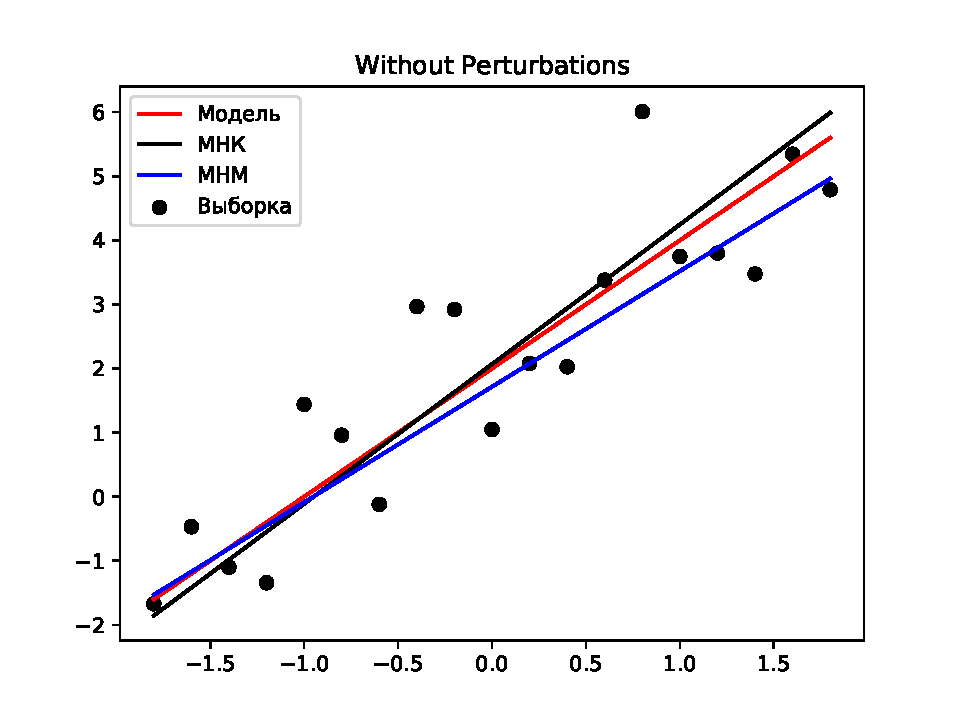
\includegraphics[width = 10cm, height = 8cm]{src/Without Perturbations}
                    \caption{Выборка без возмущений}
                    \label{without_pert}
                \end{figure}
                МНК$~distance~=~\WithoutPertLSMDistance$ \\
		        МНМ$~distance~=~\WithoutPertLMMDistance$

            \subsubsection{Выборка с возмущениями}
                \begin{enumerate}
                    \item{Критерий наименьших квадратов:}
                    $\hat{a}\approx \WithPertLSMBetaNULL$, $\hat{b}\approx \WithPertLSMBetaONE$
                    \item{Критерий наименьших модулей:}
                    $\hat{a}\approx \WithPertLMMBetaNULL$, $\hat{b}\approx \WithPertLMMBetaONE$
                \end{enumerate}
                \begin{figure}[H]
                    \centering
                    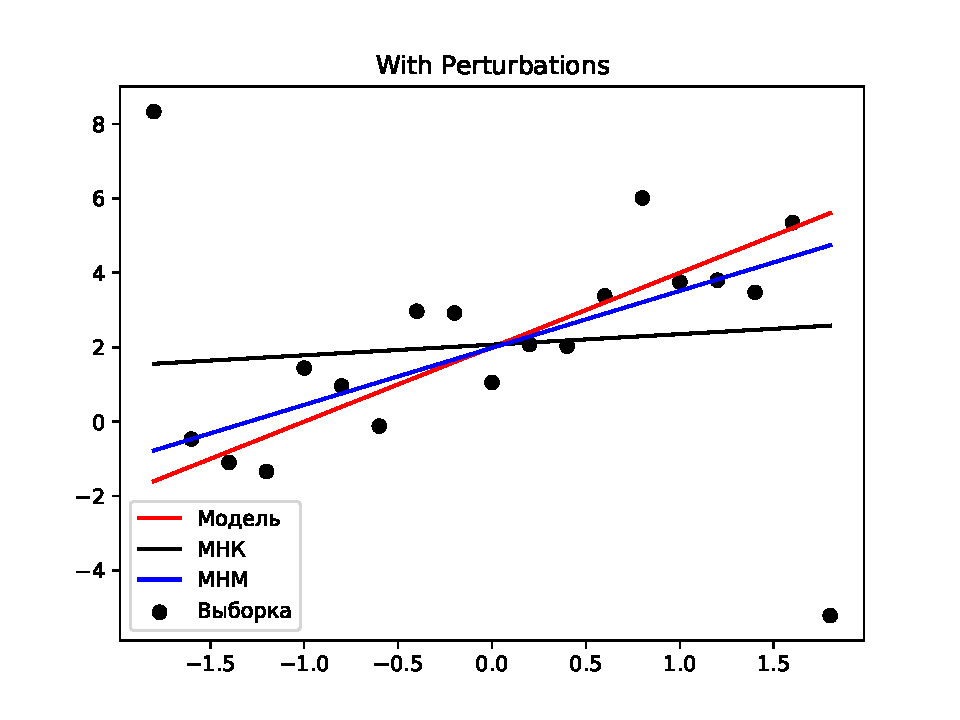
\includegraphics[width = 10cm, height = 8cm]{src/With Perturbations}
                    \caption{Выборка с возмущениями}
                    \label{with_pert}
                \end{figure}
                МНК$~distance~=~\WithPertLSMDistance$ \\
		        МНМ$~distance~=~\WithPertLMMDistance$

	\section{Обсуждение}
        Видно, что
    \section{Приложение}
        С кодом работы и отчета можно ознакомиться по ссылке:\;\url{https://github.com/sqrtyyy/MathStat/tree/master/lab_6}
\end{document}

